\documentclass{beamer} 
\usetheme{CambridgeUS}

\title{Vim}
%\subtitle{}
\author{Roberto Alvarado}
\institute{USFQ}
\date{\today}

\begin{document}

  %Title
  \begin{frame}[t]
    \maketitle
  \end{frame}

  %Table of content
  \begin{frame}[t]
    \tableofcontents
  \end{frame}

  %Introduccion
  \section{Introducción}
  \subsection{Vim y otros editores de texto}
  \begin{frame}
    \frametitle{Editores de Texto}
      Primeros editores eran en la linea de comando\\
      \begin{itemize}
        \item TECO (text-editor-\&-corrector) \\
        \item ED
      \end{itemize}
      \begin{figure}[h]
        \centering
        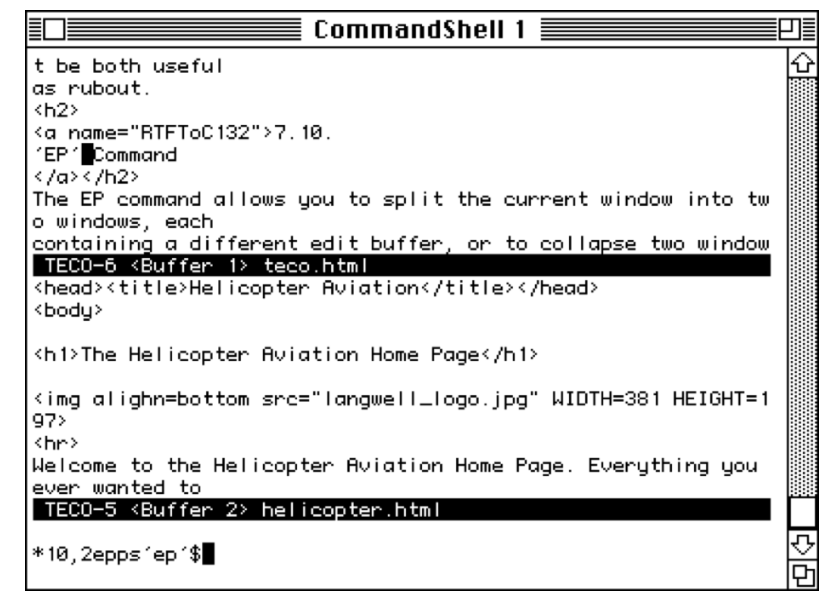
\includegraphics[width=0.4\textwidth]{./resources/1.png}
        \caption{TECO editor}
        \label{fig:1}
      \end{figure}
  \end{frame}

  \begin{frame}[t]
    \frametitle{Vim}
    \framesubtitle{Vim como editor de texto}
    Vim es una herramienta de edición de texto dentro de la linea de comando
    (en Windows funciona como aplicación), es una versión mejorada de Vi y se
    maneja en un sistema de modos (estados) y comandos.\\
    \bf{Mision de Vim}
    \begin{itemize}
      \item Minimizar el tiempo de edición 
      \item Dejar de utilizar el mouse
    \end{itemize}
      \centering
      
\includegraphics[width=0.2\textwidth]{./resources/6.png}
  \end{frame}

  \begin{frame}[t]
    \frametitle{Vi, Vim, NEOVim}
    \framesubtitle{Entendiendo la diferencia}
    \begin{table}[h]
      \centering
      \caption{Diferencias entre Vi y Vim}
      \label{tab:label}
    \begin{tabular}{|c|c|}
        \hline
        \bf{Vi} & \bf{Vim (Vi iMproved)} \\ 
        \hline
        1976 & 1991\\
        \hline
        Editor base de todo sistema LUNIX & Es una aplicación aparte\\
        \hline
        2 modos & 5 modos \\
        \hline
        Solamente editar el archivo & Implementación de facilidades \\ 
        \hline
      \end{tabular}
    \end{table}
  \end{frame}

  \begin{frame}[t]
    \frametitle{Vim vs Vi} 
    \begin{figure}[h]
      \centering
      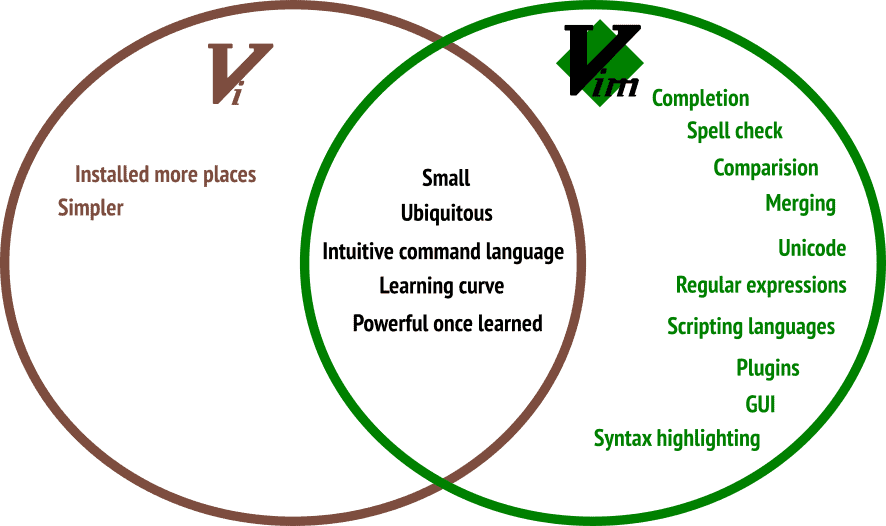
\includegraphics[width=0.8\textwidth]{./resources/5.png}
      \caption{Vi vs Vim}
      \label{fig:}
    \end{figure}
  \end{frame}

  \begin{frame}[t]
    \frametitle{Actualidad}
    \framesubtitle{Editores de texto en la actualidad}
    \begin{figure}[h]
      \centering
      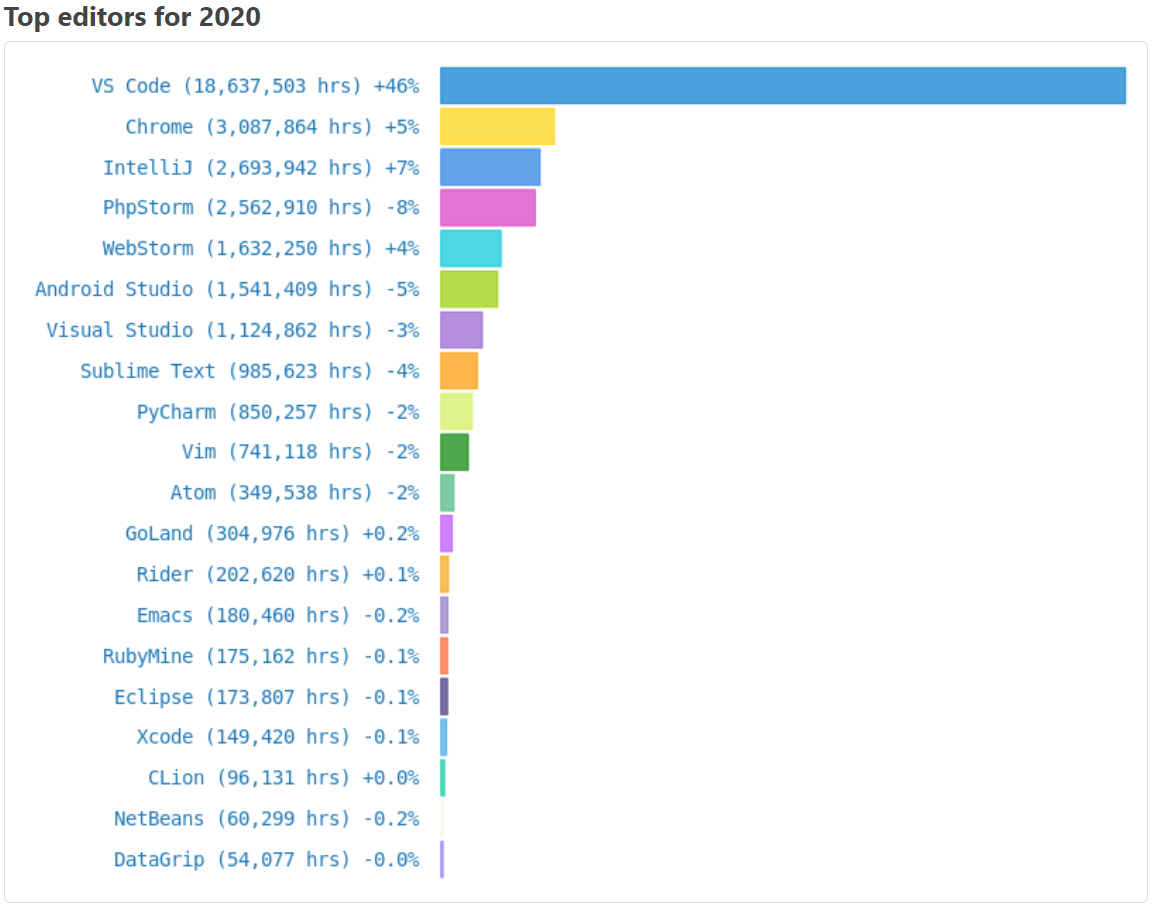
\includegraphics[width=0.5\textwidth]{./resources/4.png}
      \caption{Editores de texto en el 2020}
      \label{fig:2}
    \end{figure}
  \end{frame}

  \subsection{Mi experiencia}
  \begin{frame}[t]
    \frametitle{Mi experiencia con VIM}
    \begin{figure}[h]
      \centering
      
\includegraphics[width=0.43\textwidth]{./resources/3.png}
      \caption{The scary thing about vim}
      \label{fig:5}
    \end{figure}
  \end{frame}

  \begin{frame}[t]
    \begin{figure}[h]
      \centering
      
\includegraphics[width=0.8\textwidth]{./resources/7.png}
      \caption{Vim in a nutshell}
      \label{fig:3}
    \end{figure}
  \end{frame}
  
  \begin{frame}[t]
    \frametitle{Verdades de VIM}
    \framesubtitle{@Ben Orenstein}
    \begin{itemize}
      \item Vim no es solo para los nerds que no tienen nada que hacer
      \item Vim es sencillo de aprender, es como un juego de vídeo
      \item Con dos semanas de práctica serás más eficiente que con tu editor actual
    \end{itemize}
    \begin{figure}[h]
      \centering
      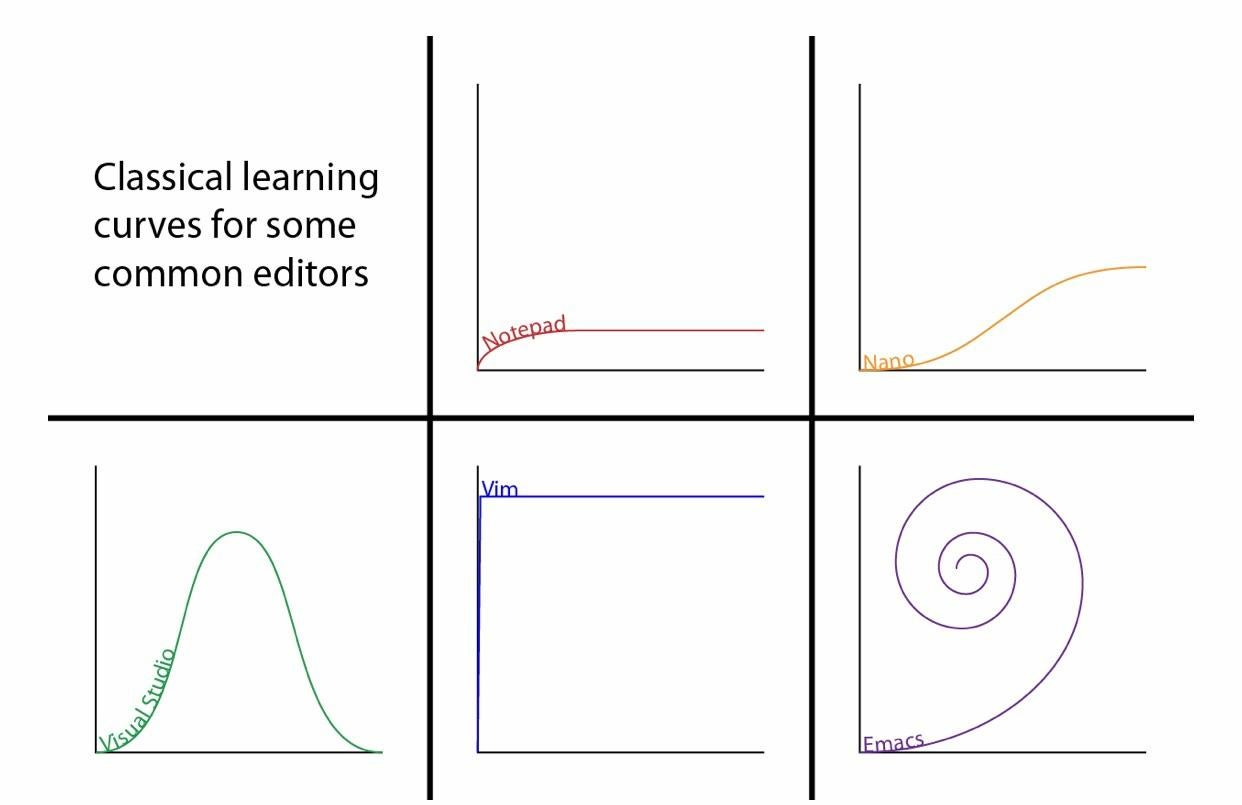
\includegraphics[width=0.6\textwidth]{./resources/8.png}
      \label{fig:7}
    \end{figure}
  \end{frame}
  \subsection{Instalar Vim}
  \begin{frame}[t]
    \bf{LINUX}
    \begin{block}{Ubuntu}
      sudo apt-get install vim
    \end{block}
    \begin{block}{Arch}
      sudo pacman -S vim
    \end{block}
    \begin{block}{Fedora}
      sudo dnf install vim
    \end{block}
    \vspace{1cm}
    \bf{MAC}
    \begin{block}{Necesario homebrew para manejo de paquetes}
      brew install vim
    \end{block}
  \end{frame}
  \begin{frame}[t]
    \bf{Windows}
    \begin{figure}[h]
      \centering
      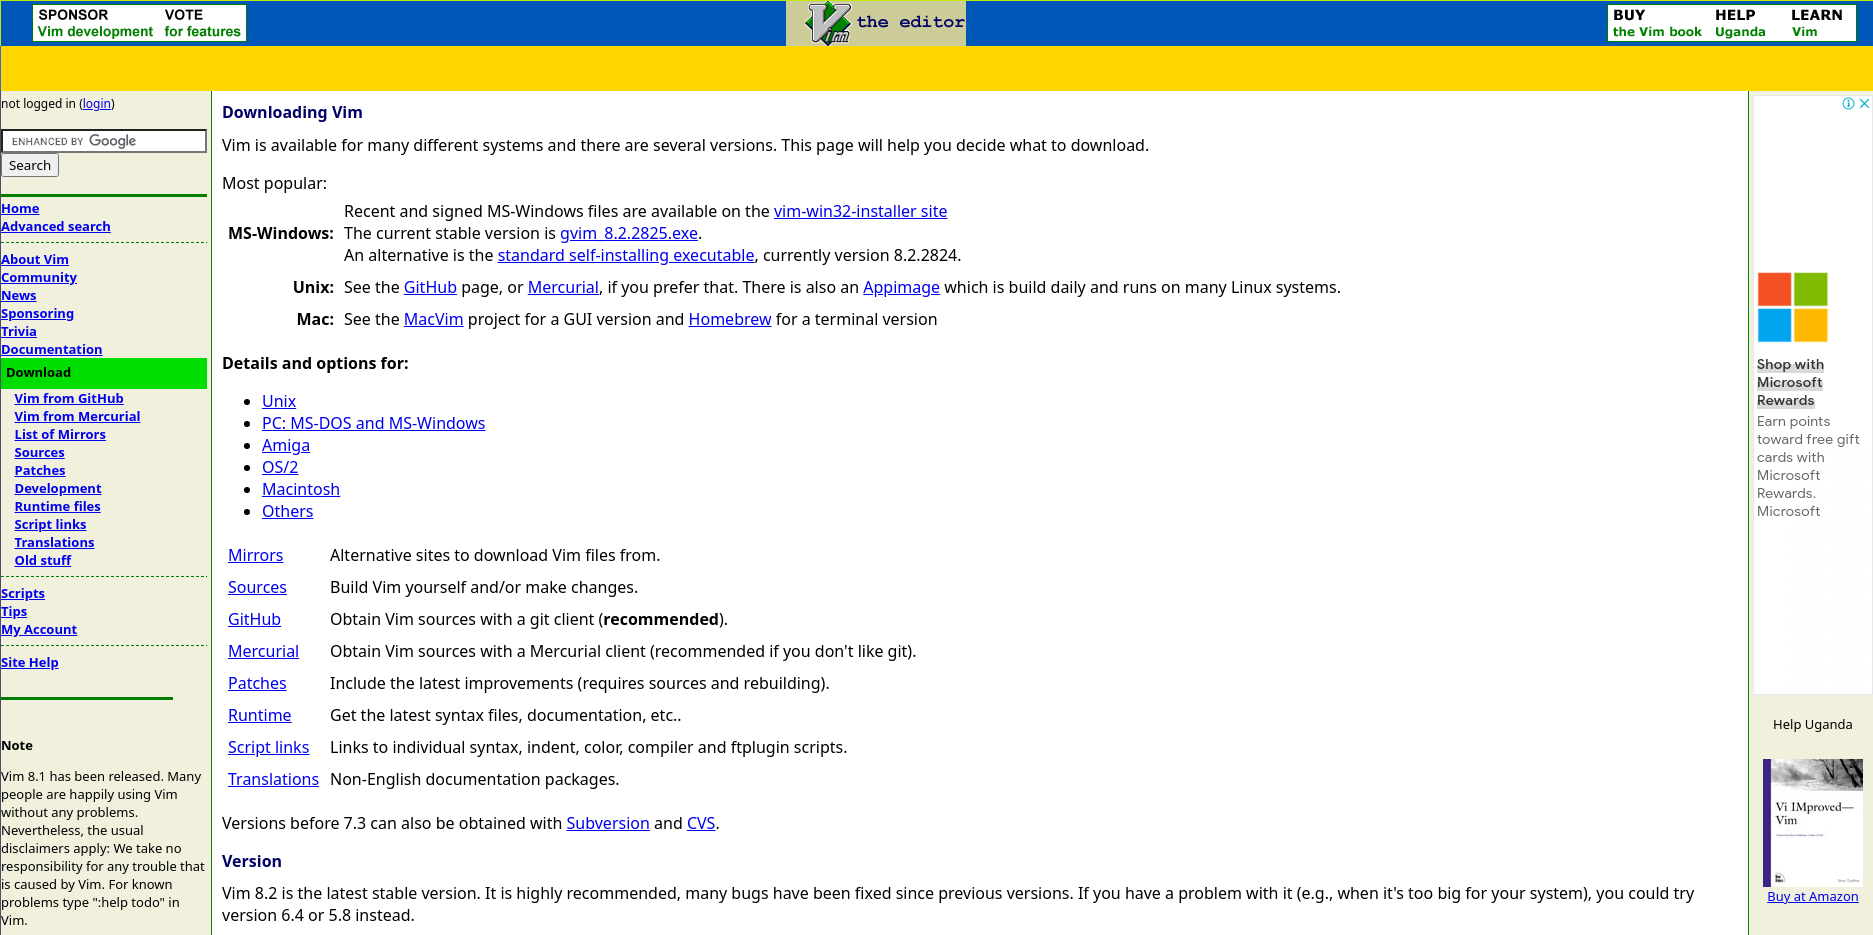
\includegraphics[width=0.9\textwidth]{./resources/9.png}
      \label{fig:9}
    \end{figure}
    \vspace{1cm}
    https://www.vim.org/download.php
  \subsection{Modos de Vim}
  \end{frame}
  \begin{frame}[t]
    \frametitle{Modos de Vim}
    \framesubtitle{Entendiendo el editor}
    Vim funciona según el modo en que se encuentre.
    Hay 3 diferentes estados
    \begin{itemize}
      \item Normal (Comandos)
      \item Insert (Insertar texto dentro del archivo)
      \item Visual (Marcar el texto como cuando se selecciona un conjunto de texto en vim)
    \end{itemize}
    \begin{figure}[h]
      \centering
      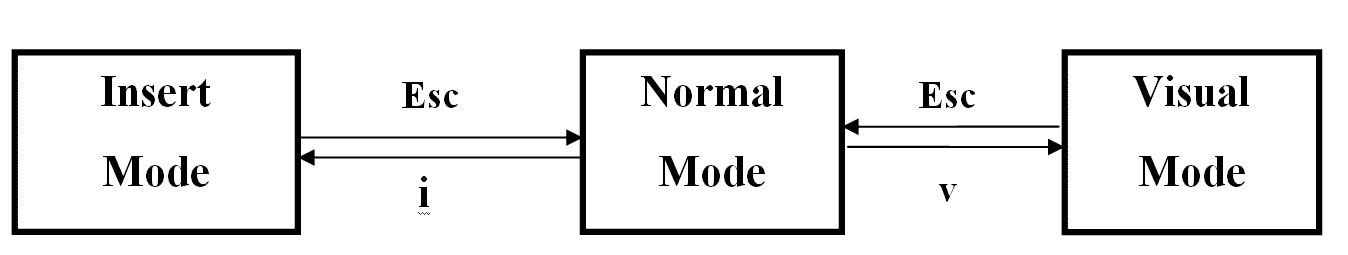
\includegraphics[width=0.8\textwidth]{./resources/10.png}
      \caption{Estados de Vim}
      \label{fig:10}
    \end{figure}
  \end{frame}
  \begin{frame}[t]
    \frametitle{Insert mode}
    \begin{itemize}
      \item Este es el modo en que menos tiempo queremos estar
      \item Este modo el editor de texto es como cualquier otro editor
      \item Cualquier cosa que escribamos se va a insertar en el archivo 
    \end{itemize}
  \end{frame}
  \begin{frame}[t]
    \frametitle{Visual mode}
    \begin{itemize}
      \item Sistema mejorado de Vi
      \item Se utiliza para marcar un area de texto
    \end{itemize}
    
  \end{frame}

\end{document}
